% ==================================================
% CHAPTER 2: The LHC and ATLAS Experiment %
% ==================================================

\chapter{The LHC and ATLAS experiment}
\label{chap:lhc_atlas}
% Edit count: Lia - 1, Brigitte - 0

%TODO : Write physics motivation as section 2.1 and adjust this chapter intro
The LHC and ATLAS experiment are introduced here to provide context for the New Small Wheel upgrade. \textcolor{red}{Adjust this based on new physics motivation section}

% --------------------------------------------------
\section{Physics Motivation}
% --------------------------------------------------
\textcolor{red}{Gotta write this}

% --------------------------------------------------
\section{The Large Hadron Collider}
% --------------------------------------------------

% Include order for inst lum.
% Include bunch crossing frequency
The LHC is an accelerator \SI{27}{\kilo\meter} in circumference and located $\sim$\SI{100}{\meter} underground at CERN near Geneva, Switzerland~\cite{evans_lhc_2008}. It has two beam pipes that counter-circulate bunches of protons\footnote{the LHC also accelerates lead ions, but this paper is written in the context of proton-proton collisions} before colliding the bunches in the center of one of four major experiments, such as the ATLAS experiment (discussed in section~\ref{sec:atlas}). There, the partons interact and many physics processes can occur. The LHC enables physicists to study particle physics at the energy frontier. In the previous run of the LHC (run-2), protons were collided with a center of mass energy of \SI{13}{\tera\electronvolt}. 

% There are two main branches of study that can be pursued with the LHC and ATLAS. First, properties predicted by the standard model (SM) of particle physics can be measured. Else, physicists can search for evidence of processes predicted by theories beyond the standard model. Both the SM measurement and search analyses are based on measuring the number of times a given process occurs and comparing it to expectations. In this way, the number of proton-proton interactions created by the LHC directly affects the statistics available to do SM measurements and searches using the ATLAS experiment.

The number of proton-proton interactions generated by the LHC directly affects the statistics available to make fundamental measurements of cross sections, event rates, etc. 
%IF YOU DON'T NEED TO DEFINE LUMINOSITY
% The number of interactions is quantified by luminosity, a property of the accelerator and its operating conditions~\cite{zyla_review_2020}. When the instantaneous luminosity is integrated over a data collection period and multiplied by the cross section of a given process, the result is the expected number of times that process occurs (so luminosity has units of inverse cross section). Since luminosity is derived from the accelerator parameters, it is the link between the machine and the statistical power of potential measurements. 
% IF YOU NEED TO DEFINE LUMINOSITY
% THIS SECTION IS NOT CITED, probably cite wiht zyla_review_2020
Predicting the number of proton-proton interactions requires defining a metric called luminosity~\cite{zyla_review_2020}. It is the number of particles an accelerator can send through a given area per unit time. It is calculated from the measurable quantities in equation~\ref{eqn:inst_lum}.

\begin{equation}
\mathcal{L} = \frac{f N_{1} N_{2} }{4 \pi \sigma_{x} \sigma_{y}}
\label{eqn:inst_lum}
\end{equation}

In equation~\ref{eqn:inst_lum}, $f$ is the frequency of the bunch crossings (\SI{25}{\nano\second}), $N_{1}$ and $N_{2}$ are the number of protons in each bunch ($\sim 10^{11}$ protons / bunch), and $\sigma_{x}$ and $\sigma_{y}$ are the RMS of the spatial distributions of the bunch. Therefore, luminosity is a property of the accelerator and its operating parameters. The design luminosity of the LHC was $10^{34}$ cm$^{-2}$s$^{-1}$. The units of luminosity are an inverse area; multiplying the luminosity by the cross section of a given process gives the expected rate for that process.

Integrating the \textit{instantaneous} luminosity (equation~\ref{eqn:inst_lum}) over a period of data collection gives the integrated luminosity,

\begin{equation}
L = \int \mathcal{L} \left( t \right) \,dt
\label{eqn:int_lum}
\end{equation}

which is related to the total number of interactions. In this way, the luminosity is the link between the accelerator and the statistical power of measurements to be made with the data collected. 

So far, the LHC provided an integrated luminosity of \SI{28.26}{\per\femto\barn} in run-1~\cite{atlas_luminosity_run1} and \SI{156}{\per\femto\barn} in run-2~\cite{atlas_luminosity_run2}, as shown in figure~\ref{fig:hl-lhc}. The HL-LHC upgrade~\cite{hl_lhc_tdr} was accepted because without increasing the luminosity of the LHC tenfold, running the accelerator will not provide significant statistical gain on measurements. Also, some systems will need repair and replacement to operate past $\sim$2020. The energy accessible at the LHC offers irreplaceable ability to study Higgs- and electroweak-sector physics~\cite{dainese_physics_2018}, so the European Strategy for Particle Physics made it a priority ``to fully exploit the physics potential of the LHC'' with ``a major luminosity upgrade''~\cite{european_strategy_for_particle_physics}. The goal is for the HL-LHC to provide an integrated luminosity of \SI{3000}{\per\femto\barn} in the 12 years following the upgrade. The luminosity actually achieved will depend on a combination of technological advances and upgrades in progress that affect the factors contributing to luminosity defined in equation~\ref{eqn:inst_lum}~\cite{hl_lhc_tdr}.


\begin{figure}
    \centering
    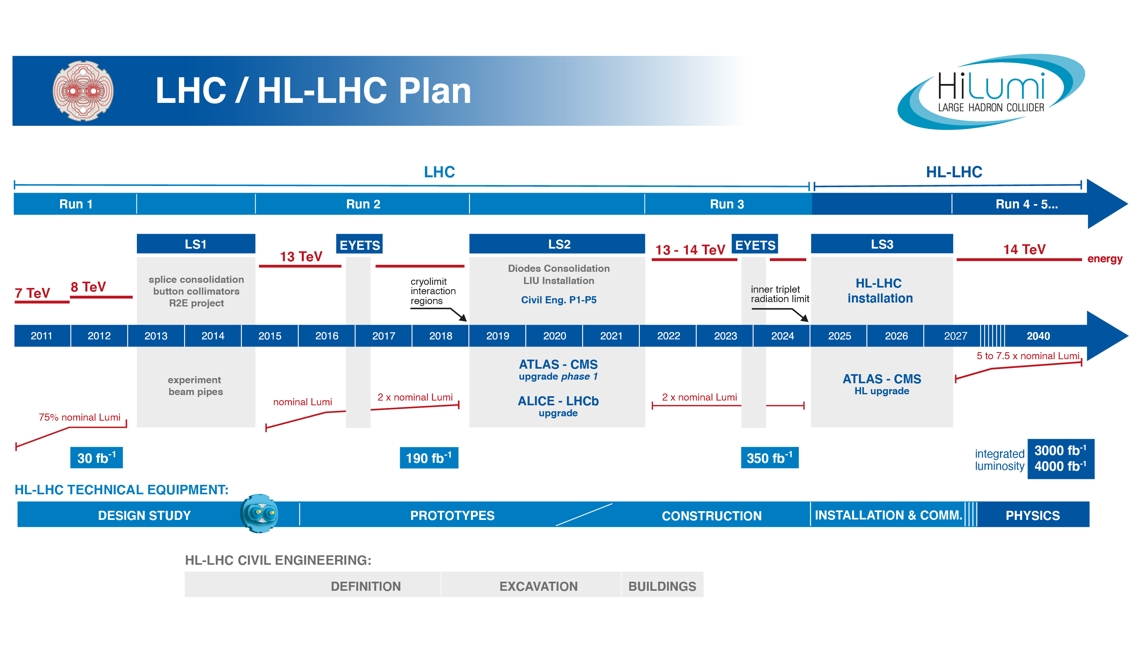
\includegraphics[width = \textwidth]{figures/HL-LHC-updated-January-2021_small.jpg}
    \caption{LHC/HL-LHC plan~\cite{hl-lhc_plan_picture_website}. The integrated luminosity collected and projected for each run of the LHC is shown in red below the timeline and the center of mass energy of the collisions is shown in red above the timeline. The top blue arrow labels the run number. ``LS'' stands for ``long shutdown'' and indicates periods where the accelerator is not operating. During the shutdowns, upgrades to the LHC and the experiments are being installed. This timeline was last updated in January, 2021, and reflects changes in the schedule due to the ongoing pandemic. }
    \label{fig:hl-lhc}
\end{figure}

%The estimated number of interactions of a given type per bunch crossing is given by equation~\ref{eqn:num_interactions}.
%\begin{equation}
%\mu = \sigma \delta t\mathcal{L}
%\label{eqn:num_interactions}
%\end{equation}

% The energies accessible by the accelerator make it unique infrastructure with which to study processes of the standard model of particle physics and search for new phenomenon beyond the standard
% model. Considerable progress has been made towards answering the questions originally used to motivate the construction of the LHC, but many remain unanswered or only partially answered~ \cite{brianti_large_1984}. Therefore, the continued use and maintenance of the accelerator 

% --------------------------------------------------
\section{The ATLAS experiment}
% --------------------------------------------------
\label{sec:atlas}

The ATLAS experiment~\cite{collaboration_atlas_2008} was designed to support all the physics goals of the LHC. It is \SI{44}{\meter} long and \SI{25}{\meter} in diameter, and weighs 7000 tones. It is an array of particle detector subsystems arranged concentrically around the beam pipe and centered around one of the LHC's interaction points (a place where the beams collide), as shown in figure~\ref{fig:atlas}. ATLAS is cylindrical because it aims to provide 4$\pi$ coverage aound the interaction point. It is helpful to separate the subsystems of ATLAS into the so-called ``barrel'' and ``endcap'' or ``forward'' regions.  % <- maybe move this sentence to muon spec section

\begin{figure}
    \centering
    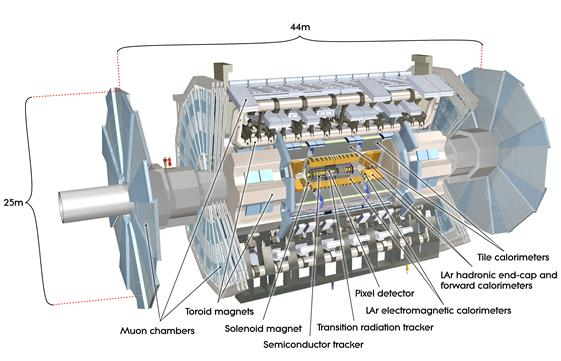
\includegraphics[width = \textwidth]{figures/atlas_diagram.png}
    \caption{Diagram of the ATLAS experiment, with the various detector subsystems labelled. Figure from~\cite{collaboration_atlas_2008}, which also contains more details about the ATLAS experiment.}
    \label{fig:atlas}
\end{figure}

For analysis, ATLAS is typically described in spherical coordinates. The azimuthal angle $\phi$ is measured around the beampipe and the polar angle $\theta$ is measured from the beam pipe. A more useful coordinate than $\theta$ is the pseudo-rapidity, $\eta = -\ln\tan\left(\theta/2\right)$, because it approaches the rapidity of a particle when its momentum is much greater than its mass and differences in rapidity are approximately invariant to a Lorentz boost parallel to the beam. The range of $\eta$ is 0 (perpendicular to the beam) to $\pm\infty$ (parallel to the beam, or the z-direction). Typically, $\eta$ is the physically interesting coordinate because the $\phi$ coordinate follows the cylindrical symmetry of the beam.

It is not actually the proton bunches that collide and generate physics processes, but their constituent partons. Since the partons may carry an unknown fraction of the momentum, ATLAS analyses are based on the sum of the transverse momentum ($p_T$) and energy of outgoing particle being approximately zero (transverse meaning perpendicular to the beam). \textcolor{red}{The goal of ATLAS is to reconstruct the transverse momentum of each collision product to understand what happened in each collision. \textit{-> Do I have this right?}} A brief overview of the sub-systems of ATLAS is given, starting from the system closest to the beam and moving outwards. Each sub-system is responsible for a different group of collision products.

\paragraph*{The inner detector} \hfill \break
The inner detector~\cite{atlas_inner_detector_tdr_1, atlas_inner_detector_tdr_2} (figure~\ref{fig:atlas_inner_detector}) is for precision tracking, vertex measurements and electron identification. A \SI{2}{\tesla} solenoid with field parallel to the beam bends the track of outgoing particles to make momentum measurements possible. The innermost part is made of high-resolution semiconductor pixel and strip detectors for precision tracking while the outermost part are straw-tubes that generate and detect transition radiation for electron identification.

\begin{figure}
    \centering
    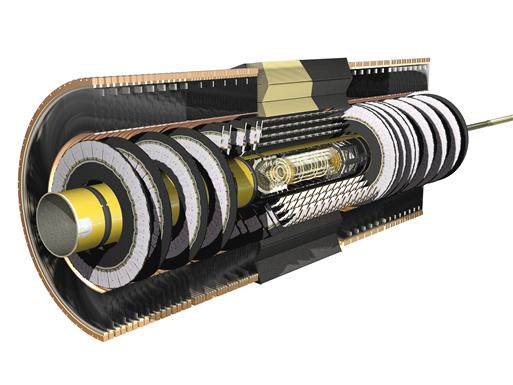
\includegraphics[width = 0.5\textwidth]{figures/atlas_inner_detector.jpg}
    \caption{Diagram of the ATLAS experiment's inner detector, with the different segments and the technology used labelled. Figure from~\cite{collaboration_atlas_2008}.}
    \label{fig:atlas_inner_detector}
\end{figure}

\paragraph*{Calorimetry system} \hfill \break
Electromagnetic and hadronic sampling calorimeter units are used to record the energy of electrons, photons, jets and missing transverse energy (from neutrinos, for example). A combination of liquid-argon (LAr) electromagnetic and hadronic calorimeters~\cite{atlas_lar_cal_tdr} and tile-scintillator hadronic calorimeters~\cite{atlas_tile_cal_tdr} cover the rapidity range $|\eta| < 4.9$, as shown in figure~\ref{fig:atlas_calorimeter}.

\begin{figure}
    \centering
    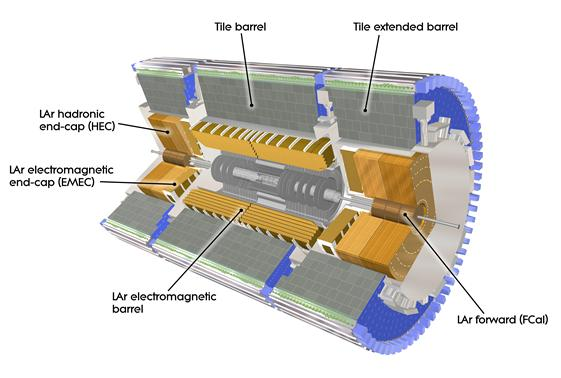
\includegraphics[width = 0.5\textwidth]{figures/atlas_calorimeter.png}
    \caption{Diagram of the ATLAS calorimeter system, with the different segments and the technology used labelled. Figure from~\cite{collaboration_atlas_2008}.}
    \label{fig:atlas_calorimeter}
\end{figure}

The calorimeters cause incoming charged particles to shower and deposit their energy in the sensitive volume. Only muons and neutrinos are known to pass the calorimeters to the muon spectrometer.  Particles other than those mentioned would have decayed in the inner detector before reaching the calorimeter. 

\paragraph*{Trigger system} \hfill \break
It would be impossible to record all the data from bunch crossings every \SI{25}{\nano\second}, corresponding to a rate of $\sim$\SI{40}{MHz}, so ATLAS has a multi-level trigger system to select events of interest for permanent storage. The Level-1 (L1) hardware trigger~\cite{atlas_l1_trigger_tdr} uses partial-granularity information from the muon spectrometer and calorimeter to trigger on high $p_T$ muons, electrons, jets, high missing transverse energy, and $\tau$ decaying to hadrons. The maximum L1 trigger rate ATLAS can accommodate is \SI{100}{kHz} with a latency of \SI{2.5}{\micro\second}. 

% The Level-1 (L1) hardware trigger uses the muon spectrometer's TGCs and RPCs to trigger on high $p_T$ muons and the calorimeter detector units to trigger on electrons, jets, high missing transverse energy, and $\tau$ decaying to hadrons, with a maximum trigger rate of \SI{100}{kHz} and latency of \SI{2.5}{\micro\second}. The L1 trigger only uses a fraction of the granularity offered by the detectors.

The L1 trigger is used to define regions of interest that are fed into the software high level trigger (HLT), in which the full granularity of the muon spectrometer and calorimeter are used with information from the inner detector to reduce the trigger rate to 1 kHz. Events that pass the L1 and HLT trigger are recorded for use in offline analysis~\cite{atlas_hlt_trigger_tdr}.

The ATLAS trigger system is described in the references above but the trigger rates quoted here are after the upgrades implemented for run-2, described in~\cite{martinez_run-2_2016}.

\paragraph*{Muon spectrometer} \hfill \break
Magnetic deflection by superconducting air-core toroid magnets is used to measure muon momentum and energy. In the barrel of ATLAS, eight coils bent into ``racetracks'' are arranged around the beampipe provide the magentic field. In the forward region, two end-cap toroids each with eight smaller racetrack-shaped coils arranged symmetrically around the beampipe are inserted in the ends of the barrel toroid~\cite{atlas_magnet_tdr}. Figure~\ref{fig:atlas_muon_spectrometer} shows the toroid magnets and the different parts of the ATLAS muon spectrometer.

\begin{figure}
\centering
\begin{subfigure}{.5\textwidth}
  \centering
  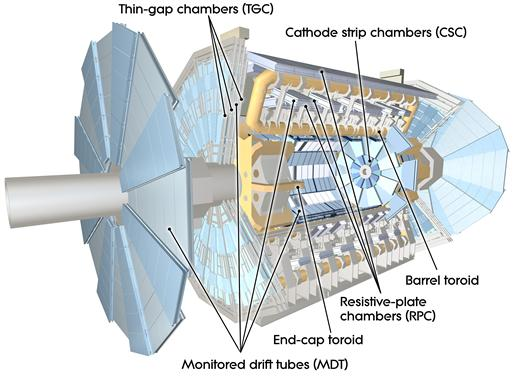
\includegraphics[width=\linewidth]{figures/atlas_muon_spectrometer.jpg}
  \caption{}
  \label{fig:atlas_muon_spectrometer_3D}
\end{subfigure}%
\begin{subfigure}{.5\textwidth}
  \centering
  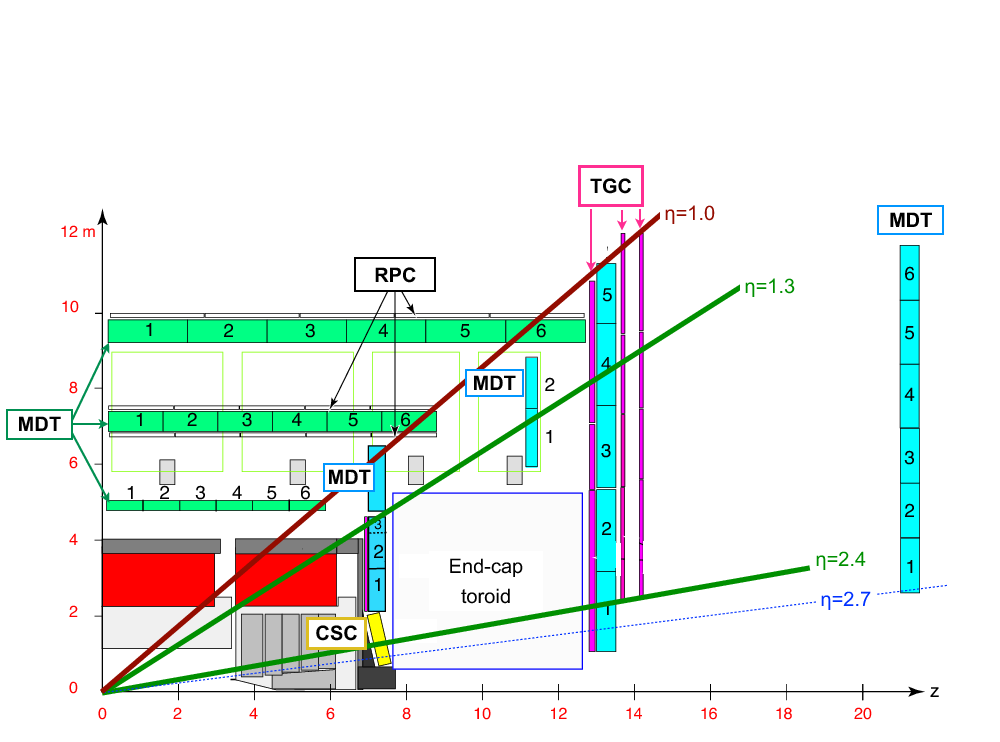
\includegraphics[width=\linewidth]{figures/atlas_old_muon_spec_quarter_cut_recolour.png}
  \caption{}
  \label{fig:atlas_muon_spectrometer_cut}
\end{subfigure}
\caption{(a) The ATLAS muon spectrometer~\cite{collaboration_atlas_2008}. (b) A quarter-cut of ATLAS, with the interaction point in the bottom left corner. The small wheel is just left of the end cap toroid, the big wheel is to its right, and the outer wheel is the rightmost structure~\cite{atlas_performance_muon_trigger_2015}}
\label{fig:atlas_muon_spectrometer}
\end{figure}

The muon spectrometer~\cite{atlas_muon_spectrometer_tdr} is separated into detectors used for precision offline tracking and for triggering. Three layers of monitored drift tubes (MDTs) or cathode strip chambers (CSCs) are used for tracking. The position of the muon track in each of the three layers allows reconstruction of the track sagitta and hence momentum. For the design momentum resolution of $\Delta p_T / p_T <$~1$\times$10$^{-4}~p$~/~GeV for $p_T <$~300~GeV and a few percent for lower $p_T$ muons, the MDTs and CSCs required position resolution of \SI{50}{\micro\meter} each. Accordingly, an optical alignment system was designed to monitor and correct for chamber positions~\cite{atlas_muon_spectrometer_tdr, aefsky_optical_2008}. 

% Precision tracking is done offline for events passing the muon trigger. Each of the barrel and encap systems have three layers of MDTs that record the position of the muon as it passes through each layer. Knowing the magentic field, the muon's momentum can be extracted. For the design momentum resolution of $\Delta p_T / p_T <$ 1$\times$10$^{-4}~p$ / GeV for $p_T < 300 GeV$ and a few percent for lower $p_T$ muons, the MDTs and CSCs required position resolution of \SI{50}{\micro\meter} each. Accordingly, an optical alignment system was designed to monitor and correct for chamber positions~\cite{atlas_muon_spectrometer_tdr, aefsky_optical_2008}. 

% ON MUON TRIGGERING IN THE ENDCAP
% Decide how you want to do this based on the next section.
% At least 2 TGC layers in coincidence comes from muon spectrometer TDR; coincidence with "forward inner" detectors (small wheel) comes from run 2 trigger upgrades paper, Martinez.
% NSW TDR says there are TGC layers in the small wheel that are the forward inner detectors added to run 2 triggering.
% \textcolor{red}{The run 2 L1 muon trigger was passed if TGC layers (two for low $p_T$ muons, three for high $p_T$ muons) of the big wheel fired in coincidence with a hit from the MDTs of the small wheel on the order of the bunch crossing time. The regions of interest defined by the TGCs were fed into the HLT, where MDT and TGC data could be combined for further cuts. The $p_T$ resolution of the L1 trigger is improved by the MDT tracking information. \textit{I'll decide how I want to do this after writing the motivation for the NSW}}
Resistive plate chambers (RPCs) are used for triggering in the barrel and thin-gap chambers (TGCs) are used for triggering in the endcaps. The positions of each type of chamber are sketched in figure~\ref{fig:atlas_muon_spectrometer_cut}. Often, the endcap muon spectrometer is separated into three wheels~-- the small wheel (SW), big wheel, and outer wheel~-- ordered by proximity to the interaction point. In run-1, low (high) $p_T$ muons were triggered on at L1 if two (three) of the RPCs or TGCs layers around the big wheel fired in coincidence, for the barrel and endcaps respectively~\cite{atlas_l1_trigger_tdr}. After run-1 it was discovered that up to 90\% of the triggers in the endcap were fake, caused by background particles generated in the material between the small wheel and the big wheel~\cite{nsw_tdr}.  To reduce the fake rate in run-2, the TGCs on the inside of the small wheel also had to register a hit. The added condition reduced the trigger rate by 50\% in the range 1.3 $< |\eta| <$ 1.9~\cite{martinez_run-2_2016}. The effectiveness of the solution was limited since the $|\eta|$-range of the small wheel TGCs was limited to 1.0 $< |\eta| <$ 1.9 and the position resolution of the small wheel TGCs is coarse~\cite{nsw_tdr}.

% In the barrel, three layers of MDTs are used for precision tracking, and resistive plate chambers (RPCs) are used for triggering. The endcaps of the muon spectrometer are composed of three wheels each, the small wheel (SW), big wheel, and outer wheel. All three wheels use MDTs for precision offline tracking, but cathode strip chambers (CSCs) are used in the forward region of the small wheel because they can better handle the increased background. Thin gap  chambers

% The big wheel and the outer wheel have MDTs for offline precision tracking and the thin gap chambers (TGCs) on either side for triggering. In the first two runs of ATLAS, offline precision tracking on the small wheel was done with MDTs and cathode strip chambers (CSCs), and their output did not contribute to the trigger.~\cite{atlas_muon_spectrometer_tdr}. 

% Sentences if you go without 1/4 cut figure
% In the barrel, three layers of monitored drift tubes (MDTs) are arranged between, above and below the barrel toroid magnets. They are used for precision tracking. On both sides of the middle layer of  MDTs and on the top of the top layer of MDTs are resitive plate chambers (RPCs), used for triggering.
%  The inner part had cathode strip chambers (CSCs), which had higher granularity to handle the increased background radiation rate in the forward region

% The muon spectrometer is the outermost layer of the ATLAS detector, since only muons (and neutrinos) can pass through the calorimeters. For muons that are ejected towards the end-caps of ATLAS, their trajectory is bent by the magentic field and their position recorded by three successive wheels of muon detectors. With each wheel providing the position of the muon along its trajectory and knowledge of the magentic field, the momentum of the muon generated in the collision can be reconstructed. 